\subsection{Cen�rio Detec��o de Dissolves \label{use_case_dissolves}}

\begin{figure}[h|top]
 \centering
 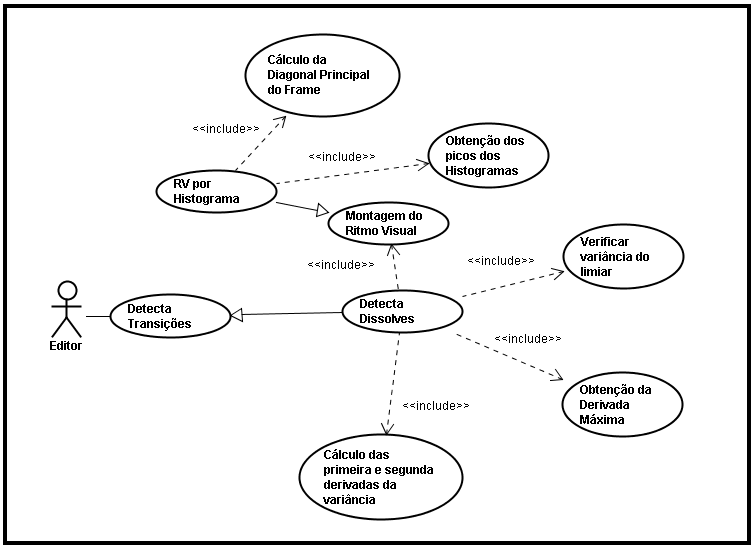
\includegraphics[width=1.0\linewidth]{imagens/use_case_dissolve.png}
 \caption{Caso de Uso para cen�rio de detec��o dos dissolves.}
 \label{img:uc_geral}
\end{figure}

\subsubsection{Caso de uso: Detecta Dissolves \label{use_case_detecta_dissolves}}

\textbf{Cen�rio Principal:} Feito o carregamento do v�deo,
executa-se os mesmos passos para a detec��o de fades, por�m, ao
final destes passos, � preciso analisar a curva da derivada m�xima
para diferenciar o dissolve do fade.


Na detec��o de fades, o pico da derivada m�xima mostra a ocorr�ncia
de fade. Para o dissolve, � preciso verificar se existe uma
seq��ncia de um pico, um vale e outro pico novamente.
